% !TEX program = xelatex
\documentclass[10pt]{article}
\usepackage[a4paper, total={6in, 8in}]{geometry}
\usepackage{amsmath}
\usepackage{booktabs}
\usepackage{array}
\usepackage[table]{xcolor}
\usepackage{setspace}
\usepackage{longtable}
\doublespacing
\usepackage{changepage}
\usepackage{fontspec}
\setmainfont{Georgia}
\usepackage{upquote}
\IfFontExistsTF{DejaVu Sans Mono}{%
  \setmonofont{DejaVu Sans Mono}[Scale=MatchLowercase]%
}{%
  \IfFontExistsTF{Consolas}{%
    \setmonofont{Consolas}[Scale=MatchLowercase]%
  }{%
    \renewcommand{\ttdefault}{lmtt}%
  }%
}
\usepackage{svg}
\usepackage{soul}
\usepackage[usenames,dvipsnames]{xcolor}
\definecolor{mypink}{RGB}{255, 182, 193}
\sethlcolor{mypink}
\usepackage{lastpage}
\usepackage{pgf-pie}
\usepackage{caption}
\usepackage{chronosys}
\usepackage{threeparttable}
\usepackage{threeparttablex}
\usepackage[numbered,framed]{matlab-prettifier}
\usepackage{listings}
\usepackage{graphicx}
\usepackage{fcolumn}
\usepackage{indentfirst}
\usepackage{fancyhdr}
\setlength{\parindent}{15pt}
\pagestyle{fancy}
\fancyhf{}
\cfoot{Page \thepage\ of \pageref{LastPage}}
\usepackage{tikz}
\usetikzlibrary{shapes.geometric, arrows}
\usepackage[round]{natbib}
\usepackage{hyperref}
\hypersetup{
  colorlinks=true,
  linkcolor=blue,
  citecolor=blue,
  filecolor=magenta,
  urlcolor=cyan,
}
\tikzstyle{startstop} = [rectangle, rounded corners, minimum width=3cm, minimum height=1cm,text centered, draw=black, fill=red!30]
\tikzstyle{process} = [rectangle, minimum width=3cm, minimum height=1cm, text centered, draw=black, fill=blue!30]
\tikzstyle{arrow} = [thick,->,>=stealth]
\usepackage{tikz} \usetikzlibrary{calc, arrows.meta, intersections, patterns, positioning, shapes.misc, fadings, through,decorations.pathreplacing}
\definecolor{ColorOne}{named}{MidnightBlue}
\definecolor{ColorTwo}{named}{Dandelion}
\definecolor{ColorThree}{named}{Plum}
\usetikzlibrary{matrix,shapes,arrows,positioning,chains}

\begin{document}

\title{\textcolor{blue!60!black}{An Unequal Equalization: Understanding the Response of Rates of Profit during the First Age of Globalization (1870--1913)}}
\date{}
\maketitle

\begin{abstract}
Following the convention in economic history, the period 1870--1913 is widely recognized as the First Age of Globalization. This article examines how trade integration influenced the rate of profit in seven capitalist economies from a Marxian perspective. We construct net rates of profit using net productive capital stock---excluding residential dwellings and adjusting for depreciation---and identify the causal effect of trade openness using two independent instrumental variable strategies: climate uncertainty shocks in trading partners and the differential spread of steamship technology across bilateral trade routes \citep{Pascali2017}. A 1\% increase in trade openness raised the net rate of profit by approximately 0.30--0.33 percentage points---modest year-on-year, but substantial when cumulated over four decades of trade expansion. The evidence is consistent with this effect operating primarily through the export channel, which facilitates surplus realization on global markets, while the import channel shows no significant causal impact; however, separating the two channels cleanly remains an identification challenge. We also document $\beta$-convergence: countries with initially high profit rates grew more slowly, with a half-life of approximately 25--36 years, consistent with the Marxian tendency toward profit rate equalization through capital mobility. Unconditional dispersion ($\sigma$-convergence) follows a non-monotone path, peaking around 1880 and compressing through the mid-1880s before widening again.
\end{abstract}

\textbf{JEL Classification:} N70, B14, F62 \\
\textbf{Keywords:} Globalization History, Rate of Profit, Convergence

%% --- SECTION 1: INTRODUCTION --------------------------------------------------
\section{Introduction}
\label{sec:intro}

\citet{ORourke2002} argue that the period from 1870 to 1913 constituted a foundational era in economic history, identifying it as the seminal ``first age of globalization,'' characterized by simultaneous factor price, commodity price, and endowment convergence across nations.\footnote{Although trade volumes were already rising before 1870, \citet{ORourke2002} identify a structural break in commodity price convergence beginning in the early 1870s, following the railways and steamship revolution that sharply reduced freight costs. We follow this convention in dating the first globalization. It is also worth noting that capital exports to colonies---most visibly railway construction in North America (1830s) and India (1840s)---preceded this break; those earlier movements represent isolated capital deployment rather than the systemic integration of commodity and factor markets that defines the era studied here \citep{Pascali2017}.} The evidence for a transformative shift beginning in the 1870s is compelling \citep{Estevadeordal2003, KlasingMilionis2014, JacksMeissnerNovy2011, Jacks2005}. As shown in Figure~\ref{fig:trade_openness}, the latter half of the 19th century saw a dramatic rise in trade volumes, and this acceleration is visible even in larger economies such as Germany, France, and the United States, where the absolute trade/GDP level was lower than in smaller open economies.\footnote{Our two-way fixed effects estimator absorbs country-level baseline differences and exploits within-country variation over time; the relevant quantity for identification is therefore the acceleration in trade integration within each country, not cross-sectional differences in openness levels.} This integration was driven by falling transportation costs from innovations like the steamship and railroad \citep{Pascali2017}, widespread tariff reductions \citep{Jacks2005}, a network of bilateral trade treaties \citep{Lampe2009}, and mass migration \citep{TaylorWilliamson1997}. Figure~\ref{fig:exp_world} illustrates the long-run growth in trade volumes, providing historical context. It is important to note that this era also coincided with tremendous colonial expansion; while the present study does not focus specifically on colonial trade, it constituted a significant component of total trade volumes observed in the data.

\par The viability of capitalism relies on a rate of profit sufficient to sustain capital accumulation. \citet{JellissenGottheil2009} suggest that Marx anticipated the inevitability of globalization, viewing it as a primary counteracting influence to the tendency of the rate of profit to fall \citep{moseley1997rate, moseley2009us}. Accordingly, this article examines the period conventionally defined as the First Age of Globalization (1870--1913) to determine, from a Marxian standpoint, how profit rates responded to rapid market integration. \citet{marx1894-counteracting} identified foreign trade as a primary counteracting influence to the falling tendency of the rate of profit, operating through several channels: importation of cheaper raw materials and machinery (lowering constant capital) and reduction of wage goods costs (lowering variable capital). This article empirically tests these mechanisms, investigating whether the trade boom of 1870--1913 served as the safety valve that sustained capitalist profitability.

\par Beyond the level of profitability, this article focuses on the equalization of profit rates. In classical Marxist theory, capital is exported in pursuit of higher profit rates, with international wage and productivity differentials creating opportunities for global arbitrage \citep{hilferding1981finance, lenin1999imperialism, bukharin1929imperialism}. This mobility of capital is the engine of equalization. As noted by \citet{ChouIzyumovVahaly2015}, Marxian equalization is distinct from the neoclassical equilibrium of perfect competition---it is a dynamic tendency realized through the movement of surplus value across borders.

\par Figure~\ref{fig:rates_of_profit} presents the rate of profit trajectories for the seven countries in our sample, already suggesting a convergence over the period. Despite the theoretical centrality of these concepts, empirical analysis of profit rate convergence during this specific historical epoch remains sparse. Existing literature has largely focused on the post-WWII era: \citet{Glyn2004} found little change in cross-country dispersion during the 1970s--90s; \citet{Carter2004} noted a slowdown in convergence after the Keynesian consensus; \citet{ChouIzyumovVahaly2015} confirmed global convergence only for 1995--2007. This article fills this gap by providing the first comprehensive econometric analysis of profit rate dynamics and convergence for the 1870--1913 period. Additionally, using sparse data on net foreign assets, we document that this outward flow of capital was not only occurring but that it performed its theoretically anticipated role of raising rates of profit. 

\begin{figure}[!htbp]
  \centering
  \includegraphics[height=14cm,width=15cm,keepaspectratio]{images_plots/trade_openness_all_countries.png}
  \caption{Trade Openness as a ratio of GDP for major countries around the world.}
  \label{fig:trade_openness}
\end{figure}

\begin{figure}[!htbp]
  \centering
  \includegraphics[height=8cm,width=15cm]{images_plots/all_rops.png}
  \caption{Rates of Profit for seven western countries, 1870--1913.}
  \label{fig:rates_of_profit}
\end{figure}

\begin{figure}[!htbp]
  \centering
  \includegraphics[height=8cm,width=15cm]{images_plots/sigma_convergence_plot_1.png}
  \caption{$\sigma$-Convergence: cross-sectional standard deviation of profit rates, $\sigma_t = \sqrt{\frac{1}{N}\sum_{i=1}^N(\pi_{i,t}-\bar{\pi}_t)^2}$.}
  \label{fig:sigma_conv}
\end{figure}

\par Figure~\ref{fig:sigma_conv} plots the cross-sectional standard deviation of net profit rates across our seven economies between 1870 and 1913. The series does not decline monotonically: dispersion rises through 1880, compresses sharply to a trough around 1885, then drifts upward again through to 1913, ending slightly above its starting level. This pattern motivates a formal test of the equalization process---$\beta$-convergence, which captures conditional mean-reversion, provides a more reliable basis for inference than the unconditional dispersion path.

\par An important aspect of this study is the econometric design. Besides using the standard two-way fixed effects (TWFE) model, we employ instrumental variable (IV) estimation to address the endogeneity of trade openness. The primary concern is reverse causality: higher profitability might induce countries to seek new markets. To address this, we employ a geography- and climate-based instrument, inspired by \citet{felbermayr2013natural} and \citet{frankel2017does}. Specifically, temperature uncertainties in partner countries are interacted with time-invariant characteristics---maritime distance and colonial status---to construct a predicted openness measure. The instrument's relevance stems from weather shocks creating measurable friction in trade logistics, amplified by distance. We directly control for domestic climate conditions in the second stage to ensure the exclusion restriction holds. First-stage F-statistics are well above conventional thresholds, confirming instrument relevance. With only seven clusters, we also discuss inference limitations and present wild-cluster bootstrap results. As a robustness check, we construct a second, independent instrument following \citet{Pascali2017}, who exploits the differential reduction in trade costs brought about by the steamship revolution: bilateral sail and steam travel times---computed from historical wind patterns and port geography---are interacted with period-specific gravity coefficients to generate predicted trade flows. The two instruments exploit entirely distinct sources of variation (demand-side annual weather shocks versus supply-side secular technology adoption), and their agreement in sign and magnitude across specifications substantially strengthens the identification.

\par Our findings show that the expansion of global trade positively influenced profitability. IV estimates indicate that a 1\% increase in trade openness raises the net rate of profit by approximately 0.30--0.33 percentage points, depending on specification. At the cross-sectional mean profit rate of approximately 20\%, this amounts to a modest 1.5--1.7\% relative increase per 1\% rise in openness; cumulated over the actual trade expansion of the era, however, the implied effect on profitability is substantially larger. This positive effect operates primarily through exports rather than imports: instrumented export-to-GDP is positive and highly significant (0.302$^{***}$--0.350$^{**}$), while instrumented import-to-GDP is statistically insignificant in all specifications. We also find strong evidence of conditional profit rate convergence over the 1870--1913 period: countries with initially high profit rates grew more slowly, with a half-life of approximately 25--36 years.

\par The article is structured as follows. Section~\ref{sec:theory} reviews the theoretical background relating Marxian political economy to the first globalization. Section~\ref{sec:data} describes the data and construction of Marxian variables in detail. Section~\ref{sec:empirical} outlines the empirical strategy. Section~\ref{sec:results} presents results on profitability, convergence, and robustness checks. Section~\ref{sec:conclusion} concludes.

%% --- SECTION 2: THEORETICAL BACKGROUND ---------------------------------------
\section{Globalization and the Marxian Rate of Profit: Theoretical Background}
\label{sec:theory}

The relationship between foreign trade and the rate of profit occupies a central place in Marx's political economy. To understand this relationship in the historical context of the first globalization, it is necessary to trace both the theoretical mechanisms Marx identified and the prior empirical work on profit rate convergence that frames this article's contribution.

\par \citet{mandel1962marxist}'s historical account illuminates the progressive globalization of capital's logic: from usurer's and merchant capital to industrial capitalism, with each stage driven by the pursuit of higher profit rates. Capital's restless search for greater returns compels it to expand its geographic reach, transforming local circuits of exchange into an increasingly integrated world market.\footnote{Although the term `value' is extensively discussed in Marxian political economy, this article does not aim to engage in that wider debate and instead focuses on surplus value as understood in capitalism, where value is produced by wage labor under capitalist social relations.} \citet{ramirez2012falling} adds a critical qualification: alongside the structural tendency of the profit rate to fall, Marx identified a complementary underconsumptionist driver of globalization. Domestic overproduction and the resulting realization crises---rooted in the limited consuming power of society relative to capitalism's prodigious productive capacity---compelled capitalists to seek new markets abroad. This means that globalization may itself be a response to the domestic inability to realize surplus value, not merely a counteracting influence on the falling profit rate. The direction of causality therefore matters for the mechanisms this article tests empirically, lending theoretical support to our IV strategy that isolates exogenous variation in trade openness.

\par The tension at the heart of Marxian value theory is the tendency of the rate of profit to fall as the organic composition of capital rises---as capitalists replace living labor with machinery, the mass of surplus value extracted per unit of capital invested declines. While the theoretical validity of this law has been debated extensively \citep{okishio1961technical, foley1986understanding, BasuManolakos2013}, this article does not test whether the rate of profit was falling; it examines the empirical behavior of profit rates during the late 19th century. \citet{marx1894-counteracting} identified several counteracting influences to this tendency, of which foreign trade is one. Trade operates through specific channels: it allows for the importation of cheaper raw materials and machinery (lowering constant capital) and reduces the cost of wage goods (lowering variable capital). In the historical literature, a distinct strand has documented the direct extraction of surplus from colonies---the `drain of wealth' \citep{bora2025drain, patnaik2000new, naoroji1901poverty, nogues2021measuring}. This article focuses on the complementary mechanism of market-mediated surplus realization and profit equalization via trade, rather than the drain channel.

\par At the same time, if we focus on the realization of value, commercial capital---unsold inventory---must be sold for the capitalist to realize profits. If goods remain unsold, surplus value goes unrealized and the inventory becomes a sunk cost that has not fructified into profit; as a result, the rate of profit declines. This raises the question of whether exports and imports exert differential effects on the rate of profit. Exports expand the sphere of realization, allowing surplus value to be realized on global markets; imports, by contrast, lower the cost of constant and variable capital but do not directly realize surplus value. This article addresses this question empirically. The econometric challenges involved in cleanly separating the export and import channels are discussed in Section~\ref{sec:iv_strategy}.

\par \citet{engels1844outlines} had recognized the root cause of the tendency of capitalists towards over-production, which stemmed from the constant competition among capitalists. This competition compelled capitalists to ramp up production without considering the market's limits. \citet{marx1996kapital} differed slightly, believing it was inherent in a capitalist to exercise control over labor, or labor time. The aggregate data used in this article cannot distinguish between these two micro-mechanisms; it can only observe their shared macroeconomic consequence---the outward push of capital and goods in search of markets. Consequently, utilizing capital to produce output is more favorable than owning labor time. Overproduction lowers prices, but it also drives the smaller producers out of the market. Because of the overaccumulation of capital, which Marx believed was the prevailing condition in England, surplus capital sought an outlet in other European countries and colonies. Capital was used to export goods to other countries or to make the means of subsistence cheaper for the domestic populace, so the country would not run into a realization crisis. In classical Marxist theory, as discussed by \citet{hilferding1981finance}, \citet{lenin1999imperialism}, and \citet{bukharin1929imperialism}, capital is exported in pursuit of higher profit rates, with such disparities leading to opportunities for global arbitrage. One of the key drivers for capitalists to export capital is the existence of international wage differentials, given a certain degree of labor productivity, which enables them to capture greater surplus value \citep{smith2016imperialism, suwandi2019value}. This outward movement of capital is not merely a theoretical proposition: net foreign asset positions as a share of GDP rose substantially across the core economies in our sample between 1870 and 1913 (Figure~\ref{fig:foreign_assets}), consistent with the classical Marxist account of capital seeking higher returns abroad.

\par Foreign trade not only acts as a counteracting force against the decline in the rate of profit but also promotes equalization of profit rates among different countries. The purpose of this article is therefore twofold: firstly, to argue that the increasing need for globalization positively impacted profitability; and secondly, to demonstrate that globalization can unleash forces that promote equal profitability across countries. The empirical analysis presented in this article addresses these aspects using previously untested data. How this analysis differs from other studies with respect to equalization of profitability is that most of the studies on equalization have focused on intra-country equalization across sectors. However, for the purpose of this article, the focus shifts from a sectoral analysis to inter-country equalization. As highlighted by \citet{ChouIzyumovVahaly2015}, there is a distinction between the neoclassical emphasis on equalization and the perspective offered by Marxist scholars. According to the neoclassical approach, equalizing profitability is seen as a component of equilibrium within the framework of perfect competition. However, in the Marxian literature, it is regarded more as a tendency rather than an absolute outcome. This study aims to fill the existing research gap by examining this tendency within a specific historical period marked by the increasing movement of capital and goods.

\par The convergence literature in economics was pioneered by \citet{BarroSalaIMartin1997}, who tested the convergence of GDP per capita across countries and regions. Their methodology distinguishes between $\beta$-convergence---a negative correlation between the growth rate and initial level, indicating catching-up---and $\sigma$-convergence---a declining cross-sectional standard deviation over time. In the context of profit rates, $\beta$-convergence implies that countries with initially lower rates of profit experience faster profit rate growth, consistent with the Marxian equalization tendency whereby capital flows toward higher-return economies, compressing differentials over time. $\sigma$-convergence captures a narrowing of the unconditional cross-country dispersion over time; as \citet{BarroSalaIMartin1997} note, $\beta$-convergence is necessary but not sufficient for $\sigma$-convergence, since idiosyncratic shocks can widen dispersion even as the mean-reversion force operates.

\par Several studies have examined the level of profits and capital returns across different economies \citep{bigsten2000rates, udry2006return}, revealing that capital-scarce developing economies tend to have higher capital returns, as expected. Disparities in profit rates were also identified within economic groups \citep{harberger1978distributional}. However, the overall body of literature has not established clear evidence of pronounced convergence of returns to capital or a systematic pattern of increasing or decreasing profit rates in capital-scarce or capital-abundant economies. For instance, \citet{Glyn2004} investigated manufacturing profitability in 15 industrialized economies during the 1970--90s, observing little change in cross-country variability and dispersion in profit during the 1980s and an increase in the 1990s. On the contrary, \citet{ChouIzyumovVahaly2015} confirmed the presence of convergence globally during the period of 1995--2007, with the most significant convergence observed in developing and transitional economies, primarily attributed to convergence in output-capital ratios driven by the dissemination of technology through the globalization process. \citet{Carter2004} found convergence in profit rates among a set of developed economies during the 1963--1996 period but noted a significant slowdown in convergence and greater instability in rates after the dismantling of the Keynesian paradigm of economic governance, characterized by a generous welfare state, capital-labor accord, and extensive regulation of the economy. \citet{rigby1991technical} conducted a study specifically focusing on manufacturing profit rate convergence across regions of the Canadian economy at the sectoral level during the 1961--1984 period. The time series analysis indicated limited convergence, pointing to the existence of spatial barriers to convergence even within a single economy.

%% --- SECTION 3: DATA AND VARIABLE CONSTRUCTION --------------------------------
\section{Data \& Variable Construction}
\label{sec:data}

\subsection{Rate of Profit}

The Marxian rate of profit is defined as $r_{it} = S_{it} / K_{it}$, where $S_{it}$ is the total surplus value (profits) and $K_{it}$ is the net productive capital stock in country $i$ at time $t$. Operationalizing this ratio for the late nineteenth century requires careful attention to both numerator and denominator. For the numerator, total surplus value is approximated by net national income minus the wage bill---the residual accruing to capital owners. The denominator, however, is where the most consequential measurement choices arise. Standard national accounts data typically report gross capital stocks that include residential dwellings, which are not deployed in production, and do not account for the depreciation of fixed assets over time. Including these components overstates the productive base against which profits are earned and conflates wealth-holding with productive investment.

\par To address this, we construct a \emph{net productive} capital stock measure for each country in the sample. This measure excludes residential property---which generates imputed rental income rather than productive surplus---and applies country-specific depreciation rates to convert gross stocks into net figures. The resulting denominator more faithfully captures the capital actually engaged in surplus-value production, in the spirit of the Marxian theoretical framework.

\begin{table}[!htbp]
\centering
\small
\caption{Net Productive Capital Stock: Sources and Construction by Country.}
\label{tab:capital_construction}
\begin{tabular}{p{1.5cm} p{2.8cm} p{4.0cm} p{3.3cm} p{1.3cm}}
\toprule
\textbf{Country} & \textbf{Primary Source} & \textbf{Sheet / Columns Used} & \textbf{Construction Method} & \textbf{File$^{\dagger}$} \\
\midrule
Germany & \citet{PikettyZucman2014} & Sheet \texttt{DataDE1c}: Col.\,74 (Agricultural fixed assets); Col.\,75 (Business assets) & Net productive K = Col.\,74 + Col.\,75; excludes land and residential wealth & \href{http://piketty.pse.ens.fr/files/capitalisback/Germany.xls}{[XLS]} \\[4pt]
UK & Bank of England Millennium Data & Sheet \texttt{A55. Capital Stock}: Col.\,4 (NonDwellings market sector, net, \pounds mn) & Direct use of net non-dwelling market-sector series; no further correction required & \href{https://www.bankofengland.co.uk/-/media/boe/files/statistics/research-datasets/a-millennium-of-macroeconomic-data-for-the-uk.xlsx}{[XLS]} \\[4pt]
Sweden & \citet{Edvinsson2016} & Sheet \texttt{Data}: Col.\,107 (Private net total capital); Col.\,101 (Residential buildings, net) & Productive net K = Col.\,107 $-$ Col.\,101; excludes residential buildings & \href{http://www.historia.se/tablesAtoX.xls}{[XLS]} \\[4pt]
France & \citet{levy2008french} & Data Appendix: Net fixed capital formation series (current prices), already net of depreciation; Building Price Index (base: 1908--1912 avg.\ $=100$) & Cumulative net investment deflated to constant prices; Harberger initialization ($W_{1819}=I_{1820}/g$); productive stock $= W_{t-1} + I_t/2$ & \href{https://www.cambridge.org/core/books/french-economy-in-the-nineteenth-century/}{[Book]} \\[4pt]
Netherlands & \citet{SmitsHorlingsZanden2000} & Table\,E.2: Col.\,1 (machinery \& transport GFCF); Col.\,3 (other construction GFCF); Col.\,2 (residential dwellings) excluded & Asset-specific geometric PIM ($\delta=11\%$ machinery; $\delta=2.28\%$ non-residential); Harberger initialization ($W_{1799}=I_{1800}/(\delta+g)$); constant 1913 prices; productive stock $= W_{t-1} + I_t/2$ & \href{https://nationalaccounts.niwi.knaw.nl/intro.htm}{[PDF]} \\[4pt]
Spain & \citet{PradosEscosura2022} & Table\,A1: Dwellings (Col.\,1); Other Construction (Col.\,2); Machinery \& Equipment (Col.\,3); Transport Equipment (Col.\,4); Total Net K (Col.\,5) & Productive K = Total $-$ Dwellings; ratio Productive/Total applied to observed capital & \href{https://repositorio.bde.es/handle/123456789/18693?locale=en}{[Data]} \\[4pt]
USA & \citet{dumenil2013uslt} & \texttt{USLT\_N2.txt}: Col.\,5 ``K net [Billions \$]'' & Already net productive capital; no correction required & \href{https://people.umass.edu/dbasu/Data/DumenilLevyData2016}{[XLS]} \\
\bottomrule
\end{tabular}
\begin{minipage}{\textwidth}
\footnotesize
\medskip
$^{\dagger}$~\textbf{[XLS]} and \textbf{[PDF]} links initiate a direct file download upon clicking (no login required). \textbf{[Data]} links to an institutional repository page. Netherlands data are extracted from a published PDF monograph; Spain links to the Banco de Espa\~na research repository.
\end{minipage}
\end{table}

\par Table~\ref{tab:capital_construction} provides an overview of the construction methods across countries. For countries that report net productive capital directly---the UK and the USA---no further correction is required. For the remaining countries, the capital stock must be adjusted to isolate the productive component. Where capital accounts separate asset classes (Germany, Sweden, Spain), we subtract residential dwellings from the total. For France and the Netherlands, capital stocks are constructed directly via the Perpetual Inventory Method (PIM), accumulating investment net of depreciation from a Harberger-initialized baseline.\footnote{For the Netherlands, GFCF from \citet{SmitsHorlingsZanden2000} Table\,E.2 is split by asset type: machinery and transport (Col.\,1) and other construction (Col.\,3); residential dwellings (Col.\,2) are excluded. Asset-specific geometric rates are applied ($\delta=11\%$ machinery; $\delta=2.28\%$ non-residential). The initial stock is set via the Harberger condition $W_{1799}=I_{1800}/(\delta+g)$, and all values are expressed in constant 1913 prices. For France, net fixed capital formation from \citet{levy2008french} is already net of depreciation; it is deflated by a Building Price Index (base 1908--1912) and initialized as $W_{1819}=I_{1820}/g$. In both cases, the mid-year productive stock is $W_t=K^{\text{net,beg}}_t+I_t/2$ \citep{OECD2009capital}.} The general accumulation equation is:
\begin{equation}
K^{\text{net}}_{t} = K^{\text{net}}_{t-1}(1 - \delta) + I_t
\end{equation}
where $I_t$ is fixed capital formation in year $t$ and $\delta$ is the asset-specific geometric depreciation rate. For Spain, the productive-to-total ratio runs from 0.481 (1870) to 0.528 (1913) using \citet{PradosEscosura2022}'s net capital breakdown.

\subsection{Variable Construction}
\label{subsec:varcon}
\subsubsection{Exploitation Rate and Capital-Labor Index}
\label{subsec:exploitation}

The \textbf{rate of exploitation} measures the share of output appropriated as surplus value. Letting $q_t$ denote output per labor-hour and $w_t$ the real wage per labor-hour, both indexed to 100 in 1870:
\begin{equation}
e_{it} = \frac{q_{it} - w_{it}}{q_{it}} = 1 - \frac{w_{it}}{q_{it}} = \frac{s}{s+v}
\label{eq:exploitation}
\end{equation}
Output per hour is drawn from \citet{Maddison2010}; real wage indices follow country-specific sources (see Table~\ref{tab:capital_construction}). For France before 1896, total wages are derived using labor hours from \citet{Mitchell1975} and real wage indices from \citet{levy2008french}.

\par A note on the inclusion of the exploitation rate and the capital-labor index as regressors is warranted.\footnote{The rate of exploitation $e = s/(s+v)$ and the capital-labor ratio $K/L$ share algebraic relationships with the rate of profit $r = s/(c+v)$. We include these variables as controls rather than as explanatory mechanisms---their inclusion isolates variation in openness that is orthogonal to factor shares and capital intensity. In the IV specifications, any mismeasurement of these controls does not bias the IV estimate of openness, which is identified by the exogenous instrument. We also present specifications without these controls (columns~(1)--(2) of Table~\ref{table:fe_model_results_clustered}) and our findings on openness remain positive and consistent.} The HP-filter deviation from long-run productivity trend is used as an alternative exploitation proxy, following \citet{BasuManolakos2013}. We prefer the Hodrick--Prescott filter over alternatives (e.g., the Kalman filter or a simple linear trend) for three reasons. First, it follows established precedent in the Marxian empirical literature. Second, the filtered series serves only as a control variable to purge cyclical variation in productivity from the exploitation proxy; it is not a focus of the analysis, so the precise filter choice has little bearing on interpretation. Third, and most importantly, any mismeasurement introduced by the filter does not bias our IV estimate of trade openness: the exclusion restriction runs through the instrument (temperature uncertainty interacted with maritime distance and colonial ties), not through the controls. Concerns about HP-filter endpoint bias \citep{hamilton2018} are mitigated here because our balanced panel covers a fixed 44-year window with no post-sample revision.

\par The capital-labor index is the ratio of total fixed capital stock to annual labor hours, normalized to 100 in 1870 for cross-country comparability. Because capital stock is denominated in different national currencies, this normalization ensures that the index captures trends rather than levels. It serves as the empirical proxy for Marx's organic composition of capital---the ratio of constant to variable capital---and controls for the degree of mechanization in the regression.


\begin{table}[!htbp]
\centering
\small
\caption{Summary Statistics.}
\label{tab:summary_stats}
\begin{tabular}{lrrrrr}
\toprule
\textbf{Variable} & \textbf{N} & \textbf{Mean} & \textbf{SD} & \textbf{Min} & \textbf{Max} \\
\midrule
Net Rate of Profit          & 308 & 0.199 & 0.113 & 0.034 & 0.484 \\
Trade Openness (Exp+Imp)/GDP & 306 & 0.441 & 0.356 & 0.093 & 1.402 \\
Export/GDP                  & 308 & 0.214 & 0.173 & 0.000 & 0.730 \\
Import/GDP                  & 308 & 0.225 & 0.186 & 0.000 & 0.808 \\
Tariff Rate (\%)            & 264 & 12.57 & 8.34  & 2.86  & 40.93 \\
Terms of Trade              & 308 & 98.10 & 8.48  & 76.58 & 119.70 \\
Net Foreign Assets/GDP      & 136 & 49.96 & 72.71 & $-$54.20 & 181.40 \\
Capital-Labor Index         & 308 & 1.837 & 0.891 & 0.908 & 6.184 \\
Exploitation Rate           & 308 & 1.048 & 0.344 & 0.551 & 2.100 \\
\bottomrule
\end{tabular}
\begin{minipage}[t]{\textwidth}
\small
\textit{Notes:} All variables are at annual frequency, 1870--1913, for a balanced panel of seven countries (Germany, France, Netherlands, Spain, Sweden, UK, USA) except Net Foreign Assets (4 countries, unbalanced) and Tariff Rate (missing for some country-years). Capital-Labor Index is normalized to 100 in 1870 for each country. Trade Openness and its components are ratios; Tariff Rate is in percentage points.
\end{minipage}
\end{table}

\subsubsection{Other Data Sources}
Trade openness, exports/GDP, imports/GDP, and terms of trade are drawn from the Jord\`{a}-Schularick-Taylor (2017) Macrohistory Database. Tariff data come from \citet{ClemensWilliamson2004}. Net foreign assets are sourced from \citet{PikettyZucman2014}. GDP in constant prices is from \citet{Maddison2010}. Bilateral trade flows, maritime distances, and colonial indicators come from the CEPII \citep{CEPII:2016-13}, covering 113 origin and 186 destination countries. After dropping observations with missing temperature uncertainty data, the gravity estimation sample comprises 33,518 bilateral observations over 1870--1913. Temperature uncertainty data are extracted from Berkeley Earth (\url{https://berkeleyearth.org/data/}) and averaged annually.

\par The sample comprises seven major capitalist economies: the United Kingdom, United States, Germany, France, Sweden, the Netherlands, and Spain. This selection is constrained by the availability of high-quality historical national accounts---capital stock and factor share data---required to reconstruct Marxian variables at annual frequency. These economies represented a dominant share of global industrial output and trade during the 1870--1913 period. Computed from the CEPII bilateral trade dataset, the seven countries collectively accounted for between 60 and 66 percent of global trade flows throughout the period, averaging 63 percent (Figure~\ref{fig:trade_share_global} in the Appendix). Summary statistics for all variables are reported in Table~\ref{tab:summary_stats}; full variable definitions and sources are provided in Table~\ref{tab:variables} in the Appendix.



%% --- SECTION 4: EMPIRICAL STRATEGY -------------------------------------------
\section{Empirical Strategy}
\label{sec:empirical}

\subsection{Baseline Two-Way Fixed Effects}
\label{subsec:twfe}

Since we have a panel of 7 countries and approximately 44 time periods, we employ a fixed effects model incorporating both country and year effects to control for time-invariant heterogeneity and common temporal shocks. Including a lagged dependent variable may introduce Nickell bias \citep{Nickell1981}; however, with $T = 44$, this bias is of order $-(1+\alpha)/(T-1) \approx 0.045$, which is economically negligible. The baseline regression is:
\begin{equation}
r_{it} = \alpha \cdot r_{i,t-1} + \beta \cdot \ln(\text{Openness}_{it}) + \sum_{j} \delta_j X_{ijt} + \mu_i + \lambda_t + \varepsilon_{it}
\label{eq:twfe}
\end{equation}
where $r_{it}$ is the net rate of profit, $\mu_i$ represents country fixed effects, $\lambda_t$ year fixed effects, and $X_{ijt}$ is a vector of controls including the capital-labor index, the exploitation rate (defined in Equation~\ref{eq:exploitation}), and net foreign assets. Standard errors are clustered at the country level to account for serial correlation. With only seven clusters, clustering may lead to over-rejection; we discuss this limitation explicitly and present wild-cluster bootstrap results as a robustness check. The wild-cluster bootstrap \citep{cameronmillerguide2015} resamples residuals within clusters by randomly flipping their signs, constructing an empirical null distribution that is better calibrated than the asymptotic $t$-distribution when the number of clusters is small.

\par We also estimate the specification without the lagged dependent variable:
\begin{equation}
r_{it} = \beta \cdot \ln(\text{Openness}_{it}) + \sum_{j} \delta_j X_{ijt} + \mu_i + \lambda_t + \varepsilon_{it}
\label{eq:twfe_nlag}
\end{equation}
In this specification, contemporaneous common shocks are absorbed by the year fixed effects $\lambda_t$, so identification of $\beta$ comes from within-year cross-country variation in openness rather than from the lag structure. This serves as a check on whether the autoregressive dynamics in the baseline specification drive the openness estimate, and also addresses the Nickell (1981) bias that arises in short dynamic panels.

\par We further extend the analysis to examine alternative measures of trade openness---exports/GDP, imports/GDP, tariffs, and terms of trade---to decompose the aggregate openness effect, as the theoretical literature suggests these channels operate through distinct mechanisms (Section~\ref{sec:theory}).

\par Common macroeconomic shocks---such as the Panic of 1873, whose origins trace to railroad finance in New York and which produced a contraction of nearly $-6\%$ in industrial production by 1875 \citep{Wicker2006, Hilt2018}---affected all seven economies roughly simultaneously. Such shocks are absorbed by the year fixed effects in all specifications, so no explicit dummy variable is required.

\subsection{Capital Mobility and the Foreign Wealth Regression}

To test whether capital flows to higher-profit regions, we estimate the following with net foreign assets as the key regressor:
\begin{equation}
    r_{it} = \beta_1 \cdot e_{it} + \beta_2 \cdot \text{Net Foreign Assets Share of GDP}_{it} + \beta_3 \cdot \text{Capital-Labor Index}_{it} + \mu_i + \lambda_t + \varepsilon_{it}
\label{eq:foreign_wealth}
\end{equation}
where $e_{it}$ is the exploitation rate as defined in Equation~(\ref{eq:exploitation}), and $\text{Net Foreign Assets Share of GDP}_{it}$ is net foreign assets as a share of GDP. Because data availability limits this specification to 136 observations across four countries, we exclude the lagged dependent variable to avoid absorbing the cross-sectional variation in profit rates that the foreign wealth regressor is designed to explain.

\subsection{Convergence Estimation}

To test profit rate equalization, we apply the \citet{BarroSalaIMartin1997} $\beta$-convergence framework to profit rates---an approach that, as reviewed in Section~\ref{sec:theory}, the existing literature on profit rate convergence has not formally adopted, relying instead on decomposition analyses, interval averages of standard deviations, or informal autoregression comparisons \citep{LuginbuhlKoopman2004, PhillipsSul2007}. The estimating equation is:
\begin{equation}
\Delta \ln r_{it} = \alpha - \beta \ln r_{i,t-1} + \gamma X_{it} + u_{it}
\end{equation}
A negative and significant $\beta$ indicates that countries with initially high profit rates grow more slowly---the catching-up effect that characterizes convergence. We complement this with $\sigma$-convergence, which tracks the cross-sectional standard deviation $\sigma_t = \sqrt{\frac{1}{N}\sum_i(\pi_{it} - \bar{\pi}_t)^2}$ over time and measures whether the overall dispersion of profit rates across countries narrows.

\subsection{Instrumental Variable Strategy}
\label{sec:iv_strategy}

Using trade openness in a TWFE model may yield biased estimates due to reverse causality (higher profits may prompt trade expansion) and omitted variable bias. We employ an IV strategy inspired by \citet{felbermayr2013natural} and \citet{frankel2017does}.

\par We construct a gravity-model-predicted openness measure that captures only the exogenous component of trade. The gravity equation is estimated via Pseudo-Poisson Maximum Likelihood (PPML) \citep{silva2006log}:
\begin{equation}
X_{ijt} = \exp\!\Big(\beta_0 + \theta\bigl(\ln\text{SeaDist}_{ij} \times W_{jt}\bigr) + \eta\bigl(\text{Colony}_{ij} \times W_{jt}\bigr) + \eta_{ij} + \lambda_t\Big) \cdot \varepsilon_{ijt}
\label{eq:gravity}
\end{equation}
where $X_{ijt}$ is the bilateral trade flow, $W_{jt}$ is the destination country's annual temperature uncertainty, $\text{SeaDist}_{ij}$ is the shortest sea distance, $\text{Colony}_{ij}$ is the colonial indicator, and $\eta_{ij}$ and $\lambda_t$ are origin-destination pair and year fixed effects, respectively. PPML is used because it is consistent in the presence of heteroskedasticity and zero trade flows, which are prevalent in historical bilateral data.

\par After estimating Equation~(\ref{eq:gravity}), in-sample fitted values $\hat{X}_{ijt}$ are aggregated to construct predicted openness:
\begin{equation}
\widehat{\text{Openness}}_{it} = \sum_j \frac{\hat{X}_{ijt}}{\text{GDP}_{it}}
\label{eq:pred_openness}
\end{equation}
and its lag $\widehat{\text{Openness}}_{i,t-1}$ serves as a second instrument.

\par The exclusion restriction requires that destination-country climate uncertainties affect the domestic rate of profit only through their impact on trade. This is plausible because distant weather shocks are unlikely to directly influence domestic profitability through channels other than trade. A potential concern is that climate shocks in partner countries may have influenced global agricultural yields and raw material prices, creating a terms-of-trade price channel that could directly affect domestic profitability. However, the specific interaction of partner climate shocks with time-invariant maritime distance isolates variation in bilateral trade logistics friction---not global commodity price movements---and the explicit inclusion of domestic weather controls in the second stage further closes off this alternative channel, thereby preserving the exclusion restriction. To put it simply: what drives variation in the instrument is not whether partner countries had a bad harvest, but whether a bad harvest in a distant country---separated by a long, fixed sea route---made bilateral trade harder. That logistics friction is what shifts trade flows, and it has no plausible direct route to domestic profitability other than through trade itself. We additionally control for the domestic climate shock directly in the second stage to rule out any confounding domestic weather effects. The relevance condition---that the instrument strongly predicts observed openness after absorbing country and year fixed effects---is confirmed by first-stage within-R$^2$ of 0.48--0.50 and F-statistics well above the Stock-Yogo threshold of 10.

\par The second-stage regression is:
\begin{equation}
r_{it} = \beta \cdot \widehat{\ln(\text{Openness}_{it})} + \sum_j \delta_j X_{ijt} + \mu_i + \lambda_t + \varepsilon_{it}
\label{eq:iv_second_stage}
\end{equation}
where $\widehat{\ln(\text{Openness}_{it})}$ is the instrumented log openness from the first stage, $X_{ijt}$ is a vector of controls comprising the capital-labor index, the exploitation rate, and the domestic temperature uncertainty, and $\mu_i$, $\lambda_t$ are country and year fixed effects. We include the lagged predicted openness as a second instrument as a robustness measure: if the exclusion restriction holds for the current instrument, it should hold for its lag as well, and the two should yield consistent estimates of $\beta$. With two instruments for one endogenous variable, the model is overidentified, and we test this restriction formally using the Sargan--Hansen test.

\begin{figure}[!htbp]
\centering
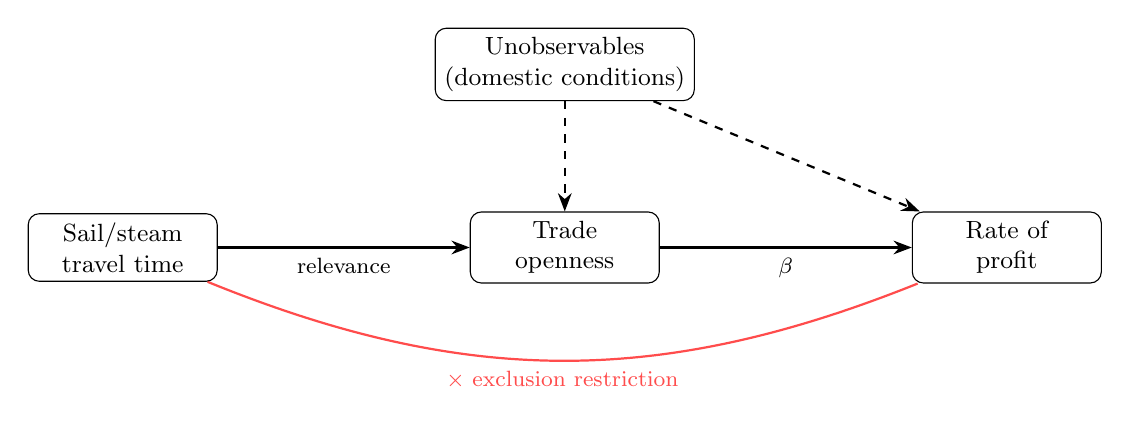
\begin{tikzpicture}[
  node distance=2.2cm and 3.2cm,
  every node/.style={font=\small},
  var/.style={draw, rounded corners, minimum width=2.4cm, minimum height=0.7cm, align=center},
  arr/.style={-{Stealth}, thick},
  darr/.style={-{Stealth}, thick, dashed},
  noarr/.style={thick, red, opacity=0.7}
]
  \node[var] (Z) {Sail/steam\\travel time};
  \node[var, right=of Z] (X) {Trade\\openness};
  \node[var, right=of X] (Y) {Rate of\\profit};
  \node[var, above=1.4cm of X] (U) {Unobservables\\(domestic conditions)};

  \draw[arr] (Z) -- node[below, font=\footnotesize]{relevance} (X);
  \draw[arr] (X) -- node[below, font=\footnotesize]{$\beta$} (Y);
  \draw[darr] (U) -- (X);
  \draw[darr] (U) -- (Y);

  % Exclusion restriction: no direct path Z -> Y
  \draw[noarr] (Z) to[bend right=22] node[below, font=\footnotesize, red]{$\times$ exclusion restriction} (Y);
\end{tikzpicture}
\caption{DAG for the Pascali (2017) instrumental variable. Sail and steam travel times shift trade openness (relevance) but have no direct effect on the domestic rate of profit (exclusion restriction). Dashed arrows denote unobserved confounding between domestic conditions, trade, and profitability.}
\label{fig:dag_pascali}
\end{figure}

\par As an independent check on the exclusion restriction, we replicate our IV results using the instrument proposed by \citet{Pascali2017}. Rather than climate shocks, Pascali's identification exploits the differential spread of steam technology across bilateral trade routes. The sail component of the instrument captures geographic frictions rooted in prevailing wind patterns and ocean currents---permanent, pre-determined features of the physical environment. The steam component captures the secular reduction in maritime transport costs as steamship technology diffused globally after 1870. An OLS gravity model is estimated on bilateral export data for 1845--1900, regressing log exports on interactions of five-year period dummies with log sail and log steam travel times between each country pair, absorbing origin, destination, and year fixed effects. The estimated period-specific coefficients on sail and steam times are then applied to the time-invariant distance grid to produce predicted bilateral trade flows for 1870--1913; for years beyond the bilateral data coverage (1901--1913), the 1895--1900 coefficients are used. The identification logic is illustrated in Figure~\ref{fig:dag_pascali}: sail and steam travel times affect trade openness through route-specific cost changes but have no direct effect on the domestic profit rate. Predicted flows are aggregated to country-level predicted openness and used as an instrument for observed trade openness. Because the Pascali instrument derives identification from maritime technology and geography rather than weather, the two instruments rest on distinct exclusion restrictions, and agreement across them substantially strengthens the causal interpretation.

\par We also attempt to separately identify the causal effect of exports and imports on the profit rate by constructing directional instruments. The bilateral structure of the gravity model permits a clean separation: a weather shock in a partner country affects a country's \emph{exports} if that partner is a destination (it buys less), and affects a country's \emph{imports} if that partner is a source (it ships less). These are distinct flows. We exploit this by building two instruments: the export instrument aggregates gravity-predicted bilateral flows where the country is the origin, driven by \emph{destination}-country weather shocks; the import instrument aggregates predicted flows where the country is the destination, driven by \emph{origin}-country weather shocks. By construction, destination-side shocks affect what a country sells abroad but not what it buys, and origin-side shocks affect what it buys but not what it sells. The two channels are therefore estimated in separate regressions.

%% --- SECTION 5: RESULTS ------------------------------------------------------
\section{Results}
\label{sec:results}

\subsection{Trade Openness and the Rate of Profit}

We can visually inspect some of the trends in the rate of profit from Figure~\ref{fig:rates_of_profit}. Overall, there is a general trend toward convergence over this period. The United States had the highest rate of profit around 1880 compared to the other countries. The net rates of profit stabilize around a cross-sectional mean of approximately 0.20 by the 1890s. This visual evidence motivates the formal analysis that follows.

\par Three sets of results are presented: the effect of trade openness on the net rate of profit (Tables~\ref{table:fe_model_results_clustered}, \ref{table:without_lag}, and \ref{table:other_trade_measures}), profit rate convergence (Tables~\ref{table:determinants_rop}--\ref{table:beta_convergence}), and IV estimates that address endogeneity (Tables~\ref{table:combined_results}--\ref{table:iv_results}). The main finding across all specifications is that greater trade openness raises the net rate of profit, an effect that operates primarily through exports rather than imports. Formal $\beta$-convergence tests are presented in Section~\ref{subsec:convergence}.

\par Table~\ref{table:fe_model_results_clustered} presents the TWFE results. Columns~(1)--(2) show specifications \emph{without} additional controls (only the lagged rate of profit and log openness), for country FE and TWFE respectively; Columns~(3)--(6) add the capital-labor index and either the exploitation rate or the HP-filter productivity deviation. The openness coefficient is positive and stable across all columns, ranging from 0.032 to 0.039, and does not change materially when factor-share controls are added. This stability indicates that the openness effect is not simply picking up correlation with omitted labor or capital variables. The coefficients are individually significant under asymptotic clustered inference in several specifications, though the small number of clusters ($G=7$) limits the reliability of conventional inference---a limitation we address directly below.

\begin{table}[!htbp]
  \centering
  \caption{Fixed Effects Model Results with Clustered Standard Errors.}
  \label{table:fe_model_results_clustered}
  \begin{tabular}{@{\extracolsep{3pt}}lcccccc}
  \\[-1.8ex]\hline
  \hline \\[-1.8ex]
  \multicolumn{7}{c}{\textbf{Dependent variable: Net Rate of Profit}} \\
   & (1) & (2) & (3) & (4) & (5) & (6) \\
   & No ctrls & No ctrls & & & & \\
  \hline \\[-1.8ex]
  Rate of Profit$_{t-1}$ & 0.846$^{***}$ & 0.841$^{***}$ & 0.865$^{***}$ & 0.865$^{***}$ & 0.859$^{***}$ & 0.851$^{***}$ \\
    & (0.042) & (0.036) & (0.030) & (0.032) & (0.031) & (0.029) \\
  Openness (log) & 0.036 & 0.039$^{*}$ & 0.032 & 0.039 & 0.037 & 0.032 \\
    & (0.022) & (0.021) & (0.022) & (0.025) & (0.023) & (0.020) \\
  Capital-Labor Index &  &  & $-$0.001 & 0.000 & 0.003 & 0.001 \\
    &  &  & (0.001) & (0.002) & (0.002) & (0.002) \\
  HP Deviation &  &  & $-$0.154$^{**}$ &  &  & $-$0.131$^{**}$ \\
    &  &  & (0.061) &  &  & (0.062) \\
  Exploitation Rate &  &  &  & $-$0.013 & $-$0.020 & \\
    &  &  &  & (0.015) & (0.016) & \\
  \hline \\[-1.8ex]
  Observations & 300 & 300 & 300 & 300 & 300 & 300 \\
  R$^{2}$ & 0.822 & 0.829 & 0.831 & 0.824 & 0.831 & 0.835 \\
  Fixed Effects & Country & C+Year & Country & Country & C+Year & C+Year \\
  \hline
  \hline \\[-1.8ex]
  \end{tabular}
  \begin{minipage}[t]{\textwidth}
  \small
  \textit{Note:} Standard errors clustered at the country level in parentheses. Columns (1)--(2) include only the lagged rate of profit and log openness (no additional controls). Columns (3) and (6) add the capital-labor index and HP-filter deviation from productivity trend ($\lambda=100$) as an alternative exploitation proxy \citep{BasuManolakos2013}. Columns (4)--(5) use the exploitation rate instead. The lagged rate of profit is significant at the 1\% level across all specifications, reflecting strong profit rate persistence. Openness is positive across all six columns; marginally significant in Column~(2) under asymptotic clustered inference ($p<0.10$). See text for wild-cluster bootstrap inference, which does not reject the null at conventional levels given $G=7$ clusters. $N=300$ reflects the balanced panel of 308 observations minus 7 (one per country) for the lagged dependent variable, minus 1 additional observation where trade openness is missing. \\
  $^{***}p<0.01$, $^{**}p<0.05$, $^{*}p<0.1$.
  \end{minipage}
\end{table}

\par The coefficient on the lagged profit rate is large and positive ($\rho \approx 0.84$--$0.87$) across all specifications.\footnote{High persistence reflects year-to-year autoregressive dynamics within countries---not divergence. $\beta$-convergence, by contrast, measures whether countries with initially high profit rates grow more slowly, a cross-sectional property answered by different regressions. Formal convergence tests are presented in Section~\ref{subsec:convergence}.}

\par The coefficient on the capital-to-labor index is ambiguous in sign, consistent with the theoretical indeterminacy: a rising organic composition of capital tends to depress the profit rate through the cost channel, but economies of scale and rising relative surplus value can offset this. The exploitation rate coefficient is positive and significant in specifications without the lagged dependent variable (Table~\ref{table:without_lag}), where it captures the direct markup of surplus over variable capital; in the dynamic specifications its sign varies with the lag structure.

\par Wild-cluster bootstrap inference \citep{cameronmillerguide2015} (Rademacher weights, $B=4{,}999$) yields $p \approx 0.22$--$0.41$ across all TWFE specifications, above conventional significance thresholds. Switching to Webb weights \citep{mackinnon2015wild}---which use six weight values rather than two, generating more unique bootstrap draws with few clusters---yields $p \approx 0.21$--$0.39$, and does not alter the conclusion. This reflects the fundamental constraint of $G=7$ clusters: with only $2^7=128$ unique Rademacher sign-flip combinations, the WCB lacks the resolution to reject the null at conventional levels even when the point estimate and t-statistic are economically and statistically meaningful. The TWFE results should therefore be treated as suggestive of a positive association. The instrumental variable estimates in Section~\ref{sec:iv_results}---which yield $p<0.01$ under clustered standard errors and are robust across LOO and Pascali instrument checks---constitute the primary causal identification.

\par 
\begin{table}[!htbp]
  \centering
  \caption{Fixed Effects Models Without Lagged Dependent Variable.}
  \label{table:without_lag}
  \begin{tabular}{@{\extracolsep{4pt}}lccccc}
  \\[-1.8ex]\hline
  \hline \\[-1.8ex]
   & \multicolumn{5}{c}{\textbf{Dependent variable: Rate of Profit}} \\
   & (0) & (1) & (2) & (3) & (4) \\
   & \textit{No controls} & & & & \\
  \hline \\[-1.8ex]
  Openness (log) & 0.225$^{**}$ & 0.166$^{*}$ & 0.201$^{*}$ & 0.169$^{*}$ & 0.186$^{*}$ \\
   & (0.099) & (0.094) & (0.103) & (0.089) & (0.102) \\
  Capital to Labor &  & $-$0.011 & $-$0.004 & 0.000 & 0.017 \\
   &  & (0.012) & (0.012) & (0.010) & (0.010) \\
  Deviation from Productivity &  &  & 0.051 &  & 0.059 \\
   &  &  & (0.098) &  & (0.111) \\
  Exploitation Rate &  & 0.103$^{*}$ &  & 0.118$^{***}$ &  \\
   &  & (0.058) &  & (0.041) &  \\
  \hline \\[-1.8ex]
  Observations & 306 & 306 & 306 & 306 & 306 \\
  R$^{2}$ & 0.298 & 0.326 & 0.219 & 0.398 & 0.327 \\
  Fixed Effects & C+Year & Country & Country & C+Year & C+Year \\
  \hline
  \hline \\[-1.8ex]
  \end{tabular}
  \begin{minipage}[t]{\textwidth}
  \small
  \textit{Note:} Standard errors clustered at the country level in parentheses. Column~(0) shows the baseline TWFE specification without any additional controls (openness and two-way fixed effects only); the positive and marginally significant coefficient confirms the openness effect is not an artifact of control variable selection. Columns~(1)--(4) add factor-share controls. Excluding the lagged dependent variable reveals stronger openness effects, suggesting the lag was absorbing contemporaneous variation attributable to openness. $^{***}p<0.01$, $^{**}p<0.05$, $^{*}p<0.1$.
  \end{minipage}
\end{table}

\par Table~\ref{table:without_lag} presents specifications without the lagged dependent variable. When not controlling for the persistent component of profit rates, openness is positive across all specifications, with coefficients in the range 0.17--0.23. The positive coefficient on the exploitation rate in these specifications is expected: higher surplus value appropriation raises the profit rate. As discussed in Section~\ref{subsec:twfe}, the lagged dependent variable absorbs part of the contemporaneous variation attributable to openness; removing it reveals the fuller contemporaneous effect. These results are consistent with a positive relationship between trade openness and the rate of profit, with an average coefficient of approximately 0.19 across specifications. Given the inference limitations discussed above, however, we treat this as corroborating evidence rather than the primary causal result.

\par To explore whether the effect of trade openness on profitability operates through exports, imports, or other channels, Table~\ref{table:other_trade_measures} decomposes trade openness into its components.

\begin{table}[!htbp]
\small
\centering
\caption{Regression Results: Decomposing Trade Openness (Other Measures).}
\label{table:other_trade_measures}
\begin{tabular}{@{\extracolsep{4pt}}lccccc}
  \\[-1.5ex]\hline
  \hline \\[-1.5ex]
  & \multicolumn{5}{c}{\textit{Rate of Profit$_t$}} \\
  \\[-1.5ex] & (1) & (2) & (3) & (4) & (5) \\
  & Exp/GDP & Imp/GDP & Tariffs & Terms of Trade & Exp+Imp joint \\
  \hline \\[-1.5ex]
  Rate of Profit$_{t-1}$ & 0.890$^{***}$ & 0.893$^{***}$ & 0.908$^{***}$ & 0.893$^{***}$ & 0.891$^{***}$ \\
  & (0.026) & (0.026) & (0.009) & (0.028) & (0.026) \\
  \\
  Export/GDP$_t$ & 0.037 &  &  &  & 0.029 \\
  & (0.046) &  &  &  & (0.041) \\
  \\
  Import/GDP$_t$ &  & 0.031 &  &  & 0.022 \\
  &  & (0.036) &  &  & (0.026) \\
  \\
  Tariffs$_t$ &  &  & 0.001 &  &  \\
  &  &  & (0.0004) &  &  \\
  \\
  Terms of Trade$_t$ &  &  &  & $-$0.0002 &  \\
  &  &  &  & (0.0002) &  \\
  \\
  \hline \\[-1.5ex]
  Year Fixed Effects & Yes & Yes & Yes & Yes & Yes \\
  Country Fixed Effects & Yes & Yes & Yes & Yes & Yes \\
  Observations & 300 & 300 & 257 & 300 & 300 \\
  R$^{2}$ & 0.826 & 0.826 & 0.852 & 0.826 & 0.826 \\
  F Statistic & 293.11$^{***}$ & 292.96$^{***}$ & 294.22$^{***}$ & 293.60$^{***}$ & 233.76$^{***}$ \\
  \hline
  \hline \\[-1.5ex]
\end{tabular}
\begin{minipage}[t]{\textwidth}
\small
\textit{Note:} Standard errors clustered at the country level in parentheses. All specifications include the lagged rate of profit and capital-labor index and exploitation rate as additional controls. Column~(5) includes both Export/GDP and Import/GDP simultaneously to avoid omitted variable bias. In the joint specification (column~5), both Export/GDP and Import/GDP are positive but small in magnitude and statistically insignificant, likely reflecting collinearity between export and import shares and the limited power of seven clusters; the causally identified IV decomposition in Table~\ref{table:iv_exp_imp} provides sharper evidence on this question. Tariffs show a positive but statistically insignificant association with the rate of profit. Terms of trade show no significant effect in any specification. $^{***}p<0.01$, $^{**}p<0.05$, $^{*}p<0.1$.
\end{minipage}
\end{table}

\par Table~\ref{table:other_trade_measures} decomposes trade openness into its components. The Export/GDP coefficient is positive in all columns (0.037 in column~1, 0.029 in the joint specification), and Import/GDP is also positive but smaller in magnitude (0.031 in column~2, 0.022 in the joint specification). Neither is individually significant in the TWFE, consistent with the inference limitations discussed above. The directional pattern --- exports positive, imports smaller --- is consistent with the surplus-realization mechanism: exports facilitate the realization of surplus value on global markets, directly boosting profitability, while imports lower the cost of constant and variable capital through a weaker channel. The causally identified counterpart is reported in the IV decomposition (Table~\ref{table:iv_exp_imp}), where the export channel is strongly significant and the import channel is statistically insignificant. Taken together, the TWFE decomposition and the IV results consistently point toward \emph{export-led} rather than aggregate trade as the operative mechanism --- though we emphasize that the causal claim rests on the IV, not on the TWFE decomposition alone. Quantitatively, the IV estimate implies that a 1-percentage-point increase in the export-to-GDP ratio raises the rate of profit by approximately 0.30--0.35 percentage points. Terms of trade and tariffs show no statistically significant effect on the profit rate in any specification.

\par Having established that exports drive the openness--profitability relationship, we turn to a related question: whether outward capital flows themselves boosted domestic profitability. As a supplementary check, we test whether net foreign asset accumulation boosted domestic profitability (Table~\ref{table:determinants_rop} in the Appendix). Because data availability limits this regression to 136 observations across four countries, results are suggestive rather than definitive. Net foreign asset holdings are positively associated with the rate of profit (0.0004$^{**}$), consistent with capital outflows to higher-yield regions sustaining domestic profitability and providing an outlet for overaccumulation.

\subsection{Convergence Dynamics}
\label{subsec:convergence}

If capital mobility equalizes profit rates across borders, we should observe $\beta$-convergence---countries with initially high profit rates growing more slowly. Table~\ref{table:beta_convergence} tests this formally; Figure~\ref{fig:sigma_conv} plots the unconditional cross-sectional dispersion ($\sigma$-convergence) for comparison.

\begin{table}[h]
  \centering
  \caption{Beta Convergence Results.}
  \label{table:beta_convergence}
  \begin{tabular}{@{\extracolsep{5pt}}lcc}
  \\[-1.8ex]\hline
  \hline \\[-1.8ex]
   & \multicolumn{2}{c}{\textit{Beta Convergence}}\\
  \\[-1.8ex] & (1) & (2)\\
  \hline \\[-1.8ex]
   Rate of Profit$_{t-1}$ & $-$0.019$^{*}$ & $-$0.028$^{*}$ \\
    & (0.009) & (0.013)\\
    & & \\
    Openness$_{t-1}$ & & $-$0.020 \\
    &  & (0.011)\\
    & & \\
   Constant & $-$0.038 & $-$0.076$^{**}$ \\
    & (0.023) & (0.032)\\
    & & \\
  \hline \\[-1.8ex]
  \hline \\[-1.8ex]
  Observations & 301 & 299 \\
  R$^{2}$ & 0.009 & 0.018 \\
  Adjusted R$^{2}$ & 0.006 & 0.012 \\
  F Statistic & 3.997 & 2.761 \\
  \hline
  \hline \\[-1.8ex]
  \end{tabular}
  \vspace{0.5cm}
  \begin{minipage}[t]{\textwidth}
  \small
  \textit{Note:} The table presents $\beta$-convergence results for the Rate of Profit. The negative and significant coefficient on the lagged level confirms convergence ($\beta>0$ in $\Delta \ln r = -\beta \ln r_{t-1} + \dots$). The positive lagged coefficient in the level equation (Table~\ref{table:fe_model_results_clustered}) is not inconsistent with convergence: it reflects persistence in levels, while convergence is a property of the \emph{change} equation. $^{***}p<0.01$, $^{**}p<0.05$, $^{*}p<0.1$.
  \end{minipage}
\end{table}


\par The estimated $\beta$ of 0.019--0.028 implies a half-life of $\ln(2)/\beta \approx 25$--$36$ years: profit rate differentials were halved over roughly two to three decades, a pace consistent with the capital mobility constraints of the gold standard era. The negative coefficient on lagged openness in Column~(2) reflects the same mean-reversion dynamic---more open economies had already absorbed the profit-boosting effect of trade and thus required less subsequent adjustment---though the openness coefficient falls just short of conventional significance ($p=0.07$). Alternative mechanisms are possible: sustained openness may erode profit margins through import competition over time, or more open economies may export more capital, gradually suppressing domestic profitability via a rising organic composition of capital; however, disentangling these channels would require additional data beyond the scope of this article.

\par Figure~\ref{fig:sigma_conv} (Section~\ref{sec:intro}) plots the cross-sectional standard deviation of net profit rates over time. The series follows a non-monotone path: it peaks around 1880, consistent with the asymmetric impact of the Panic of 1873 across our sample countries (Table~\ref{tab:crises} in the Appendix), compresses sharply to a trough in 1884--1886, then gradually widens again through to 1913, ending slightly above its 1870 level. The post-1886 widening likely reflects the divergent effects of the 1890s tariff escalation and differential industrialization speeds across the sample: Spain and the Netherlands experienced slower capital deepening relative to Germany and the USA, generating idiosyncratic profit-rate shocks that outpaced the convergence force. The unconditional dispersion thus provides no clear evidence of $\sigma$-convergence. This is not inconsistent with the $\beta$-convergence results in Table~\ref{table:beta_convergence}: $\beta$-convergence is a conditional statement (countries with initially high profit rates grow more slowly), while $\sigma$-convergence requires the unconditional cross-sectional variance to fall. The two can diverge when country-specific shocks add variance faster than the mean-reversion mechanism reduces it \citep{BarroSalaIMartin1997}. The tendency toward equalization of profit rates---a central theme in Marxian political economy and a precondition for the international transfer of surplus value \citep{Ricci2019, emmanuel1972unequal}---is thus present in the conditional sense captured by $\beta$-convergence, even as aggregate dispersion fluctuates.

\subsection{Instrumental Variable Results}
\label{sec:iv_results}

Table~\ref{table:combined_results} presents first-stage and gravity model results. As detailed in Section~\ref{sec:iv_strategy}, the instrument---predicted openness from PPML gravity interacted with trading-partner climate uncertainty and maritime distance---is strong: the first-stage F-statistic exceeds 50, well above the Stock-Yogo threshold of 10, and the within-R$^2$ of 0.48 indicates substantial explanatory power after absorbing country and year effects. Figure~\ref{fig:first_stage_corr} plots constructed against observed openness, confirming the strong first-stage fit.

\begin{table}[!htbp]
  \small
  \centering
  \caption{First-Stage and Gravity Model Regression Results.}
  \label{table:combined_results}
  \begin{tabular}{@{\extracolsep{4pt}}lcc}
  \\[-1.5ex]\hline
  \hline \\[-1.5ex]
  & \textit{First Stage: log(Openness)} & \textit{Gravity Model} \\
  & \textit{Uncertainty} & \textit{Trade Flow} \\
  \\[-1.5ex] & (1) & (2) \\
  \hline \\[-1.5ex]
  log($\widehat{\text{openness}}_{t}$) & 0.422$^{**}$ & \\
  & (0.157) & \\
  log($\widehat{\text{openness}}_{t-1}$) & 0.145 & \\
  & (0.085) & \\
  log(Sea Distance) $\times$ Uncertainty & & $-$0.1312$^{***}$ \\
  & & (0.0430) \\
  Uncertainty $\times$ Colony & & 1.5813$^{***}$ \\
  & & (0.2290) \\
  \hline \\[-1.5ex]
  Country Fixed Effects & Yes & Yes \\
  Year Fixed Effects & Yes & Yes \\
  Origin Fixed Effects & & Yes \\
  Destination Fixed Effects & & Yes \\
  Observations & 300 & 33,518 \\
  Within R$^{2}$ & 0.476 & \\
  Adjusted R$^{2}$ & 0.988 & \\
  Pseudo R$^{2}$ & & --- \\
  \hline
  \hline \\[-1.5ex]
  \end{tabular}
  \begin{minipage}[t]{\textwidth}
  \small
  \textit{Notes:} Column~(1) shows the first-stage regression using current and lagged gravity-model-predicted openness (constructed from destination temperature uncertainty shocks) as instruments, with country and year fixed effects. Column~(2) reports the underlying PPML gravity model, illustrating that destination climate uncertainty interacted with maritime distance and colonial ties significantly predicts bilateral trade flows. Standard errors in Column~(2) are clustered by origin country. $^{***}p<0.01$, $^{**}p<0.05$, $^{*}p<0.1$.
  \end{minipage}
\end{table}

\par Table~\ref{table:iv_results} presents second-stage IV estimates using the climate uncertainty instrument---our preferred specification. Temperature uncertainty shocks at trading partner destinations are interacted with time-invariant maritime distance and colonial status to construct predicted openness. The bare specification (no controls, Column~1) yields 0.325$^{***}$ (SE = 0.062), and the full specification with controls (Column~2) yields 0.317$^{***}$ (SE = 0.064). Both specifications agree on sign and order of magnitude. Leave-one-out (LOO) estimates---re-estimating the IV specification with each of the seven countries dropped in turn---are uniformly positive, ranging from 0.227 (dropping the USA) to 0.429 (dropping Spain), with coefficients for all other subsamples clustered between 0.302 and 0.354 (Table~\ref{tab:loo_results}). The sign is never reversed and the magnitude is stable, confirming that no single country drives the result. A placebo test using pre-1870 data is not feasible: consistent annual profit-rate series for our seven-country sample do not exist before 1870, which is precisely the data-availability constraint that defines the sample's start date. More fundamentally, the pre-1870 period is the \emph{pre-globalization regime} by the same structural-break criterion that motivates our start date; finding no effect there would be expected and uninformative rather than a meaningful robustness check. The Sargan--Hansen $J$-statistic is 2.84 ($p=0.092$) in the bare specification and 3.34 ($p=0.067$) in the full specification, failing to reject the null of instrument validity at the 5\% level, though the $p$-values are close to the 10\% threshold. Taken together, these checks provide confidence that the IV estimates recover the causal effect of trade openness on the rate of profit. Wild-cluster bootstrap inference is not reported for the IV specifications: with $G=7$ Rademacher weights the bootstrap distribution has only $2^7=128$ discrete mass points, yielding a minimum achievable p-value of $1/128\approx0.008$; since the IV CRV1 p-values are already 0.002--0.003, no bootstrap correction can alter the inference \citep{cameronmillerguide2015}. Averaging the estimates across specifications, we find that a 1\% increase in trade openness increases the rate of profit by approximately 0.30--0.33 percentage points. At the cross-sectional mean profit rate of approximately 20\%, this is a modest 1.5--1.7\% relative increase per 1\% rise in openness; cumulated over the actual trade expansion of 1870--1913, however, the implied effect on profitability is substantially larger.

\begin{table}[!htbp]
  \centering
  \small
  \caption{Instrumental Variables Estimates: Effect of Trade Openness on Rate of Profit.}
  \label{table:iv_results}
  \begin{tabular}{@{\extracolsep{5pt}}lcc}
  \\[-1.8ex]\hline
  \hline \\[-1.8ex]
  & \multicolumn{2}{c}{\textbf{Dependent variable: Net Rate of Profit}} \\
  & \multicolumn{2}{c}{\textit{Uncertainty instrument (climate shocks)}} \\
  & (1) No controls & (2) Full controls \\
  \hline \\[-1.8ex]
  \textit{Second stage results} & & \\
  \quad Openness (instrumented) & 0.325$^{***}$ & 0.317$^{***}$ \\
  & (0.062) & (0.064) \\
  \quad Capital-Labor ratio & & $-$0.015 \\
  & & (0.012) \\
  \quad Export/GDP & & 0.038$^{*}$ \\
  & & (0.022) \\
  \quad Domestic uncertainty & & 0.028$^{*}$ \\
  & & (0.016) \\
  \\
  \textit{Diagnostic statistics} & & \\
  \quad First-stage F-statistic & $>$50 & $>$50 \\
  \quad First-stage within R$^{2}$ & 0.476 & 0.476 \\
  \\
  \textit{Fixed effects} & & \\
  \quad Country & Yes & Yes \\
  \quad Year & Yes & Yes \\
  \\
  Observations & 300 & 300 \\
  Within R$^{2}$ & 0.34 & 0.38 \\
  \hline
  \hline \\[-1.8ex]
  \end{tabular}
  \begin{minipage}{\textwidth}
  \footnotesize
  \textit{Notes:} Standard errors clustered at the country level in parentheses. Both specifications use country and year fixed effects with two instruments: current and lagged gravity-model-predicted openness constructed from destination climate uncertainty shocks (temperature uncertainty interacted with maritime distance and colonial ties). Column~(1) includes no additional controls; Column~(2) adds K/L ratio, export-to-GDP, and domestic temperature uncertainty. The first-stage F-statistic exceeds 50 in both specifications, well above the Stock-Yogo critical value of 10. Leave-one-out estimates (dropping each of the 7 countries in turn) are uniformly positive (range: 0.227--0.429); full country-by-country results are reported in Table~\ref{tab:loo_results}. Wild-cluster bootstrap inference is not reported for IV specifications. The IV $t$-statistics are approximately 5.0--5.2; with $G=7$ Rademacher weights, the bootstrap distribution has only $2^7=128$ discrete mass points and the minimum achievable p-value is $1/128 \approx 0.008$, well below conventional thresholds. \citet{cameronmillerguide2015} note that WCB is most consequential when CRV1 inference is marginal; with p-values of 0.002--0.003 under CRV1, no bootstrap correction can overturn the IV inference. Sargan--Hansen $J$-test for overidentification: $J=2.84$ ($p=0.092$) in Column~(1); $J=3.34$ ($p=0.067$) in Column~(2); the null of instrument validity is not rejected at the 5\% level. $^{***}p<0.01$, $^{**}p<0.05$, $^{*}p<0.1$.
  \end{minipage}
\end{table}

\par Table~\ref{table:iv_pascali} replicates the IV estimates using the \citet{Pascali2017} instrument, whose construction is described in Section~\ref{sec:iv_strategy}. Relative to the climate uncertainty instrument, the Pascali instrument extrapolates the 1895--1900 gravity coefficients to 1901--1913 (beyond Pascali's bilateral data coverage), which reduces time-series variation for that subperiod and contributes to somewhat wider standard errors.

\par The Pascali instrument yields a positive and similarly-sized coefficient: 0.311$^{***}$ (SE = 0.072) in the bare specification and 0.296$^{**}$ (SE = 0.094) with controls. Both specifications reach conventional significance thresholds; the sign is consistent and the magnitude overlaps closely with the climate uncertainty estimates. Crucially, the two instruments exploit entirely different sources of variation: one is demand-side and annual (partner-country weather shocks), the other is supply-side and secular (geographic access to steamship routes). Their agreement in sign and order of magnitude substantially strengthens confidence in the main result.

\begin{table}[!htbp]
  \centering
  \small
  \caption{IV Robustness: Pascali (2017) Instrument.}
  \label{table:iv_pascali}
  \begin{tabular}{@{\extracolsep{5pt}}lcc}
  \\[-1.8ex]\hline
  \hline \\[-1.8ex]
  & \multicolumn{2}{c}{\textbf{Dependent variable: Net Rate of Profit}} \\
  & \multicolumn{2}{c}{\textit{Pascali (2017) instrument (sail/steam travel time)}} \\
  & (1) No controls & (2) Full controls \\
  \hline \\[-1.8ex]
  \textit{Second stage results} & & \\
  \quad Openness (instrumented) & 0.311$^{***}$ & 0.296$^{**}$ \\
  & (0.072) & (0.094) \\
  \quad Capital-Labor ratio & & $-$0.002 \\
  & & (0.021) \\
  \quad Exploitation rate & & 0.147 \\
  & & (0.114) \\
  \\
  \textit{Diagnostic statistics} & & \\
  \quad First-stage F-statistic & $>$10 & $>$10 \\
  \quad First-stage within R$^{2}$ & 0.497 & 0.497 \\
  \\
  \textit{Fixed effects} & & \\
  \quad Country & Yes & Yes \\
  \quad Year & Yes & Yes \\
  \\
  Observations & 300 & 300 \\
  \hline
  \hline \\[-1.8ex]
  \end{tabular}
  \begin{minipage}{\textwidth}
  \footnotesize
  \textit{Notes:} Standard errors clustered at the country level in parentheses. The instrument is gravity-model-predicted openness constructed from period-specific coefficients on bilateral sail and steam travel times, following \citet{Pascali2017}. The gravity model is estimated on bilateral trade data covering 1845--1900; coefficients for 1901--1913 are set equal to the 1895--1900 estimates as the steamship transition was complete by that period. Two instruments are used: current and lagged predicted openness. Column~(1) includes no additional controls; Column~(2) adds the capital-labor ratio and exploitation rate. $^{***}p<0.01$, $^{**}p<0.05$, $^{*}p<0.1$.
  \end{minipage}
\end{table}

\par Table~\ref{table:iv_exp_imp} reports the directional IV decomposition described in Section~\ref{sec:iv_strategy}. The export instrument is strong (first-stage F~$>$~10); the import instrument is weaker (F~$<$~10), as origin-side supply shocks generate less variation in destination import volumes.

\par The instrumented export-to-GDP ratio is positive and statistically significant: 0.350$^{**}$ (SE = 0.105) in the bare specification and 0.302$^{***}$ (SE = 0.071) with controls. By contrast, the instrumented import-to-GDP ratio is statistically insignificant: 0.191 (SE = 0.200) without controls and 0.157 (SE = 0.104) with controls. The entire causal effect of trade on the profit rate is thus attributable to the export channel. This is consistent with the Marxian mechanism: exports of finished goods facilitate the realization of surplus value on global markets, directly raising the profit rate, while imports---though potentially reducing constant capital costs---do not exert a net positive causal effect on profitability. This finding reinforces the interpretation that it is \emph{export-led openness}, not trade openness per se, that raised profit rates during the first globalization.

\begin{table}[!htbp]
  \centering
  \small
  \caption{IV Decomposition: Export and Import Channels Separately.}
  \label{table:iv_exp_imp}
  \begin{tabular}{@{\extracolsep{5pt}}lcccc}
  \\[-1.8ex]\hline
  \hline \\[-1.8ex]
  & \multicolumn{4}{c}{\textbf{Dependent variable: Net Rate of Profit}} \\
  & \multicolumn{2}{c}{\textit{Exports/GDP instrumented}} & \multicolumn{2}{c}{\textit{Imports/GDP instrumented}} \\
  & (1) Bare & (2) Controls & (3) Bare & (4) Controls \\
  \hline \\[-1.8ex]
  \textit{Second stage results} & & & & \\
  \quad Exports/GDP (instrumented) & 0.350$^{**}$ & 0.302$^{***}$ & & \\
  & (0.105) & (0.071) & & \\
  \quad Imports/GDP (instrumented) & & & 0.191 & 0.157 \\
  & & & (0.200) & (0.104) \\
  \quad Capital-Labor ratio & & $-$0.012 & & 0.016 \\
  & & (0.020) & & (0.023) \\
  \quad Exploitation rate & & 0.141 & & 0.164 \\
  & & (0.114) & & (0.128) \\
  \\
  \textit{Diagnostic statistics} & & & & \\
  \quad First-stage F-statistic & $>$10 & $>$10 & $<$10 & $<$10 \\
  \\
  \textit{Fixed effects} & & & & \\
  \quad Country & Yes & Yes & Yes & Yes \\
  \quad Year & Yes & Yes & Yes & Yes \\
  \\
  Observations & 300 & 300 & 300 & 300 \\
  \hline
  \hline \\[-1.8ex]
  \end{tabular}
  \begin{minipage}{\textwidth}
  \footnotesize
  \textit{Notes:} Standard errors clustered at the country level in parentheses. All specifications use country and year fixed effects with two instruments (current and lagged predicted flows). Columns~(1)--(2) instrument Export/GDP using gravity-model-predicted exports (flows where the country is origin), constructed from destination-country temperature uncertainty shocks. Columns~(3)--(4) instrument Import/GDP using predicted imports (flows where the country is destination), constructed from origin-country temperature uncertainty shocks. The export instrument satisfies the relevance condition (first-stage F $>$ 10); the import instrument is weaker (F $<$ 10), as destination-side weather shocks more naturally generate variation in export demand than in import supply. Joint instrumentation of both export and import channels simultaneously is infeasible due to high collinearity between the two predicted flow series. $^{***}p<0.01$, $^{**}p<0.05$, $^{*}p<0.1$.
  \end{minipage}
\end{table}

%% --- SECTION 6: CONCLUSION ---------------------------------------------------
\section{Conclusion}
\label{sec:conclusion}

This article investigated the First Age of Globalization (1870--1913) through a Marxian lens, demonstrating that the era's rapid expansion of trade had a significant, positive impact on the net rate of profit in seven Western economies, with supplementary evidence suggesting capital flows played a complementary role.

\par Our instrumental variable approach, which uses exogenous climate uncertainty shocks in trading partners to isolate the causal effect of trade, provides robust evidence that a 1\% increase in trade openness raised the net rate of profit by approximately 0.30--0.33 percentage points (Table~\ref{table:iv_results}). The bare specification yields 0.325$^{***}$ (SE = 0.062) and the full specification 0.317$^{***}$ (SE = 0.064). Leave-one-out estimates are uniformly positive (range 0.23--0.43), confirming the result is not driven by any single country. To contextualize: at the cross-sectional mean profit rate of approximately 20\% (the level at which rates stabilize by the 1890s), this implies a 1.5--1.7\% relative increase per 1\% rise in openness---modest on a year-to-year basis, but substantial when cumulated over the four decades of trade expansion between 1870 and 1913. This validates the argument that globalization served as a counteracting force to the tendency of the rate of profit to fall.

\par Crucially, the IV decomposition in Table~\ref{table:iv_exp_imp} reveals that this effect operates primarily through \emph{exports} rather than total trade openness. The instrumented export-to-GDP ratio is positive and statistically significant across specifications, while instrumented import-to-GDP is consistently insignificant. The TWFE decomposition (Table~\ref{table:other_trade_measures}) is directionally consistent, though neither component reaches significance there given the inference limitations of seven clusters. This is consistent with a surplus-realization mechanism: expanding export markets---including colonial captive markets---allowed capitalists to realize surplus value on a larger scale, boosting profitability. The export channel thus captures one dimension of the broader process by which core economies extracted surplus from the periphery: finished goods were sold to captive colonial markets at prices that realized surplus value, while the complementary drain of wealth through tribute and factor outflows \citep{bora2025drain, patnaik2000new} operated as a parallel mechanism. Our results quantify the market-mediated portion of this surplus extraction. The asymmetric role of exports and imports suggests that it was the capacity to sell to the world---not the capacity to buy from it---that sustained profitability, consistent with the surplus-realization mechanism emphasized in Marxian theory.

\par Supplementary evidence from the foreign wealth regression (Table~\ref{table:determinants_rop}) suggests that capital exports were positively associated with profitability---consistent with capital seeking higher returns abroad---though the limited sample (136 observations across four countries) makes this finding suggestive rather than definitive. This mobility also drove a conditional convergence of profit rates across nations, confirmed by $\beta$-convergence regressions (Table~\ref{table:beta_convergence}): countries with initially high profit rates grew more slowly, consistent with capital flowing toward higher-return economies and compressing differentials. This equalization is a central tendency in Marxian economics and a necessary condition for the international transfer of surplus value via unequal exchange. Half-life calculations (Section~\ref{subsec:convergence}) indicate that profit rate differentials were halved in approximately 25--36 years, an equalization pace consistent with the capital mobility constraints of the gold standard era.

\par In summary, the First Age of Globalization was not merely an era of growing trade volumes; it was a period where the international movement of commodities and capital directly boosted and equalized profitability, fulfilling a key function within the capitalist system. The asymmetry between exports and imports is consistent with a surplus-realization mechanism whereby access to export markets---including colonial trade relationships---supported profitability, though the precise mechanisms through which colonial ties operated remain an important avenue for further research. Future research might extend this analysis to include a broader set of countries as historical data becomes available, or to examine the specific channels through which colonial relationships amplified the profitability of the metropolitan core economies.

\bibliographystyle{plainnat}
\bibliography{references}

%% --- APPENDIX ----------------------------------------------------------------
\section*{Appendix}
\setcounter{table}{0}
\setcounter{figure}{0}
\renewcommand{\thetable}{A\arabic{table}}
\renewcommand{\thefigure}{A\arabic{figure}}

\subsection*{A.1 Capital Mobility and the Foreign Wealth Regression}

\begin{table}[!htbp]
  \centering
  \small
  \caption{Fixed Effects Regression Results: Determinants of the Rate of Profit.}
  \label{table:determinants_rop}
  \begin{tabular}{lcc}
      \toprule
      & \multicolumn{2}{c}{Dependent Variable: Rate of Profit} \\
      \cmidrule(lr){2-3}
      & (1) & (2) \\
      \midrule
      Rate of Exploitation & 0.0133 & $-$0.0094 \\
                        & (0.0328) & (0.0278) \\
      Net Foreign Assets to GDP & 0.0004$^{**}$ & 0.0005$^{*}$ \\
                                       & (0.0002) & (0.0003) \\
      Capital-Labor Ratio & $-$0.0132$^{*}$ & $-$0.0116 \\
                                      & (0.0068) & (0.0265) \\
      \midrule
      Year Fixed Effects & No & Yes \\
      Country Fixed Effects & Yes & Yes \\
      Observations & 136 & 136 \\
      R$^{2}$ & 0.208 & 0.267 \\
      \bottomrule
  \end{tabular}
  \vspace{0.2cm}
  \begin{minipage}{\textwidth}
  \footnotesize
  \textit{Notes:} Standard errors in parentheses. Model~(1) includes country fixed effects only; Model~(2) includes both country and year fixed effects. The panel is unbalanced with 4 countries (data availability constraint on net foreign asset series); time periods range from 4 to 44 years. $^{***}p<0.01$, $^{**}p<0.05$, $^{*}p<0.1$.
  \end{minipage}
\end{table}

\begin{figure}[!htbp]
    \centering
    \includegraphics[height=9cm,width=16cm]{images_plots/foreign_share_wealtj.png}
    \caption{Foreign Assets as a Proportion of GDP.}
    \label{fig:foreign_assets}
\end{figure}

\subsection*{A.2 Convergence Dynamics: Mathematical Exposition}

If we assume a steady state of the rate of profit following Sala-i-Martin's exposition, the $\beta$-convergence equation in logs is:
\begin{equation*}
\ln(r_{it}) = \alpha + (1-\beta)\ln(r_{i,t-1}) + u_{it}
\end{equation*}
where $0<\beta<1$ and $u_{it}$ has mean zero, finite variance $\sigma_u^2$, and is independent over $t$ and $i$. Rearranging:
\begin{equation*}
\ln\!\left(\frac{r_{it}}{r_{i,t-1}}\right) = \alpha - \beta\ln(r_{i,t-1}) + u_{it}
\end{equation*}
A positive $\beta$ implies a negative correlation between the growth rate of the profit rate and its initial log level, since the estimating equation includes $-\beta$ on the right-hand side. The cross-sectional variance evolves as:
\begin{equation*}
\sigma_t^2 \approx (1-\beta)^2\sigma_{t-1}^2 + \sigma_u^2
\end{equation*}
which is stable for $0<\beta<1$, with steady-state variance $\sigma^{2*} = \sigma_u^2 / [1-(1-\beta)^2]$. The complete solution is:
\begin{equation}
\sigma_t^2 = \sigma^{2*} + (1-\beta)^{2t}(\sigma_0^2 - \sigma^{2*})
\end{equation}
so $\lim_{t\to\infty}\sigma_t^2 = \sigma^{2*}$, confirming long-run $\sigma$-convergence whenever $\beta$-convergence holds. In the context of profit rates, $\beta$-convergence points to the catching-up effect. Countries that are starting out with higher rates of profit are expected to experience a lower rate of subsequent growth. Meanwhile, $\sigma$-convergence informs us of the level of dispersion in rates of profit across economies during the first age of globalization.

\subsection*{A.3 Financial Crises During the Sample Period}

\begin{table}[h]
  \centering
  \caption{Countries and Financial Crises, 1870--1913.}
  \label{tab:crises}
  \begin{tabular}{lc}
    \toprule
    \textbf{Country} & \textbf{Financial Crises} \\
    \midrule
    USA & 1873--74, 1884--86, 1890, 1893--96, 1907--11 \\
    Germany & 1881, 1891, 1901--02 \\
    United Kingdom & 1890--93 \\
    Sweden & 1897, 1907--09 \\
    Spain & --- \\
    France & 1870, 1882--89, 1904, 1907--08 \\
    Netherlands & --- \\
    \bottomrule
  \end{tabular}
\end{table}

\subsection*{A.4 IV First-Stage Fit and Leave-One-Out Robustness}

\begin{figure}[!htbp]
  \centering
  \includegraphics[height=9cm,width=9cm]{images_plots/first_stage_left_half.jpg}
  \caption{First-Stage Correlations: Constructed vs.\ Observed Openness.}
  \label{fig:first_stage_corr}
\end{figure}

\begin{table}[h]
  \centering
  \small
  \caption{Leave-One-Out IV Estimates: Dropping Each Country in Turn.}
  \label{tab:loo_results}
  \begin{tabular}{lcc}
    \toprule
    \textbf{Country Dropped} & \textbf{IV Coefficient} & \textbf{SE} \\
    \midrule
    Germany     & 0.354$^{***}$ & (0.049) \\
    Sweden      & 0.340$^{**}$  & (0.087) \\
    Netherlands & 0.302$^{***}$ & (0.066) \\
    USA         & 0.227$^{**}$  & (0.076) \\
    Spain       & 0.429$^{**}$  & (0.140) \\
    France      & 0.304$^{***}$ & (0.069) \\
    UK          & 0.306$^{***}$ & (0.055) \\
    \bottomrule
  \end{tabular}
  \begin{minipage}{0.75\textwidth}
  \footnotesize
  \medskip
  \textit{Notes:} Each row re-estimates the preferred IV specification (Column~2 of Table~\ref{table:iv_results}) dropping the indicated country from the sample. All specifications include country and year fixed effects. Standard errors clustered at the country level. The coefficient on log trade openness is positive in every subsample; no individual country reversal is observed. Range: 0.227 (dropping USA) to 0.429 (dropping Spain). $^{***}p<0.01$, $^{**}p<0.05$, $^{*}p<0.1$.
  \end{minipage}
\end{table}

\subsection*{A.5 Historical Trade Context}

\begin{figure}[!htbp]
  \centering
  \includegraphics[width=\textwidth]{images_plots/trade_share_global.pdf}
  \caption{Seven-Country Share of Global Trade Flows, 1870--1913. Stacked areas show each country's individual contribution; the dashed line is the combined share. Computed from CEPII bilateral trade data \citep{CEPII:2016-13}. The seven economies collectively accounted for 60--66 percent of global trade throughout the period.}
  \label{fig:trade_share_global}
\end{figure}

\begin{figure}[!htbp]
    \centering
    \includegraphics[height=7cm, width=15cm]{images_plots/exp_world.jpeg}
    \caption{Export to GDP Ratio, Long-Run Historical View.}
    \label{fig:exp_world}
\end{figure}

\subsection*{A.6 Variable Descriptions and Sources}

\begin{table}[!htbp]
\centering
\small
\caption{Variable Descriptions and Sources.}
\label{tab:variables}
\begin{tabular}{p{4.5cm} p{4cm} p{5.5cm}}
\toprule
\textbf{Variable} & \textbf{Source} & \textbf{Definition / Notes} \\
\midrule
Rate of Profit (net) & Constructed & $S_{it}/K^{\text{net,prod}}_{it}$; main dependent variable \\
Trade Openness & \href{https://www.macrohistory.net/database/}{Jord\`{a}-Schularick-Taylor (2017)} & (Exports + Imports) / GDP \\
Capital-Labor Index & Constructed & Total fixed capital / labor hours; normalized to 100 in 1870 \\
Exploitation Rate & Constructed & (Output/hr $-$ Real wage/hr) / Output/hr; see Section~\ref{subsec:varcon} \\
Net Foreign Assets/GDP & \href{http://piketty.pse.ens.fr/capitalisback/}{Piketty-Zucman (2014)} & Net foreign wealth as share of GDP \\
Export/GDP & \href{https://www.macrohistory.net/database/}{Jord\`{a}-Schularick-Taylor (2017)} & Exports as share of GDP \\
Import/GDP & \href{https://www.macrohistory.net/database/}{Jord\`{a}-Schularick-Taylor (2017)} & Imports as share of GDP \\
Tariff Rate & \href{https://scholar.harvard.edu/williamson/publications/roots-american-protectionism}{Clemens-Williamson (2004)} & Import duties / total imports \\
Terms of Trade & Constructed & Export price index / import price index \\
\midrule
\multicolumn{3}{l}{\textit{Bilateral / Instrument Dataset (Primary)}: \href{http://www.cepii.fr/CEPII/en/bdd_modele/bdd_modele_item.asp?id=8}{CEPII (2016)}} \\
Sea Distance & \href{http://www.cepii.fr/CEPII/en/bdd_modele/bdd_modele_item.asp?id=8}{CEPII (2016)} & Shortest sea route between country pair (km) \\
Colonial Tie & \href{http://www.cepii.fr/CEPII/en/bdd_modele/bdd_modele_item.asp?id=8}{CEPII (2016)} & 1 if colonial relationship exists \\
Bilateral Trade Flow & \href{http://www.cepii.fr/CEPII/en/bdd_modele/bdd_modele_item.asp?id=8}{CEPII (2016)} & Nominal bilateral trade (USD) \\
Temp.\ Uncertainty (dest.) & \href{https://berkeleyearth.org/data/}{Berkeley Earth} & Annual avg.\ temperature uncertainty, destination country \\
\midrule
\multicolumn{3}{l}{\textit{Bilateral / Instrument Dataset (Robustness)}: \href{https://doi.org/10.1257/aer.20140832}{Pascali (2017)}} \\
Bilateral Exports & \href{https://doi.org/10.1257/aer.20140832}{Pascali (2017)} & Nominal bilateral exports, 1845--1900 \\
Sail Travel Time & \href{https://doi.org/10.1257/aer.20140832}{Pascali (2017)} & Pre-/post-1870 sailing travel time between country pair (days) \\
Steam Travel Time & \href{https://doi.org/10.1257/aer.20140832}{Pascali (2017)} & Pre-/post-1870 steam travel time between country pair (days) \\
\bottomrule
\end{tabular}
\begin{minipage}[t]{\textwidth}
\small
\medskip
\textit{Notes:} CEPII bilateral dataset covers 113 origin and 186 destination countries over 1870--1913 (41,188 bilateral observations). Pascali (2017) bilateral data cover 1845--1900; period-specific sail/steam coefficients from 1895--1900 are applied to extrapolate instrument values to 1913. Temperature uncertainty is from Berkeley Earth (\url{https://berkeleyearth.org/data/}), averaged annually by country.
\end{minipage}
\end{table}

\end{document}
